\section{The Web as a Platform} \label{chapter2:web-as-a-platform}

% \begin{wrapfigure}{R}{0.2\textwidth}
%   % \vspace{-27pt}
%   \centering
%   % \vspace{-20pt}
% \end{wrapfigure}

\marginfig{16}{0.45\textwidth}{
  \includegraphics[width=0.25\textwidth]{../resources/Mac-PC.png}
}

Similarly to operating systems, the Web browser started as a software product with extension capabilities that transformed it into a platform. % with scripts and applications.
% The distribution of an application is limited only by the platform it can be deployed on.
The Web spreads the scalability of software distribution world wide with a near zero latency.
It eventually became the main distribution medium, and the wider market there can possibly be for software.
It led the Web to become a major platform, replacing operating systems.

Now, with web applications, the distribution medium is so transparent that owning a software product to have an easier access is no longer relevant.
It stimulates a disruptive business model based on an instantaneous and free access for the user, while claiming value for their data.
This thesis focuses not on this buisness model, but rather on the technologies that brought it.
% The next paragraphs present Javascript, the language that allowed this new business model to emerge.

\subsection{The Language of the Web}

In the 80's, reducing development time became more profitable than reducing hardware costs.
% with Moore's law predicting exponential increase in hardware performance,
Higher-level languages replaced lower-level languages.
The economical gain in development time brought by productive languages compensated the decrease in performance.
Most of the now popular programming languages were released at this time, Python in 1991, Ruby in 1993, Java in 1994, PHP and Javascript in 1995.

With the democratisation of programming, the involvement of a community became critical for the adoption, evolution and maturation of a language.
Communities adopt a language because it allows to quickly experiment and enter businesses sectors.
The industry adopts a language because it responds to business needs and its community represents a hiring pool.
The community support and the industrial needs are reinforcing each other in a loop.

Java thrived in the software industry, but lose the hype that drove the community innovation and creativity.
Now, it struggles to keep up with the latest trends in software development.
On the contrary, Ruby on Rails emerged from an industrial context, but is now open source, and backed by a strong community that makes it evolve and mature.
Other languages like Python and PHP, emerged within a strong community, and were later adopted by the industry for web development.
Django, the Python web frameworks, is used to develop many web applications in industrial contexts.
The Wordpress publishing platform is another example of an economical success with PHP.

\marginfig{20}{0.5\textwidth}{
  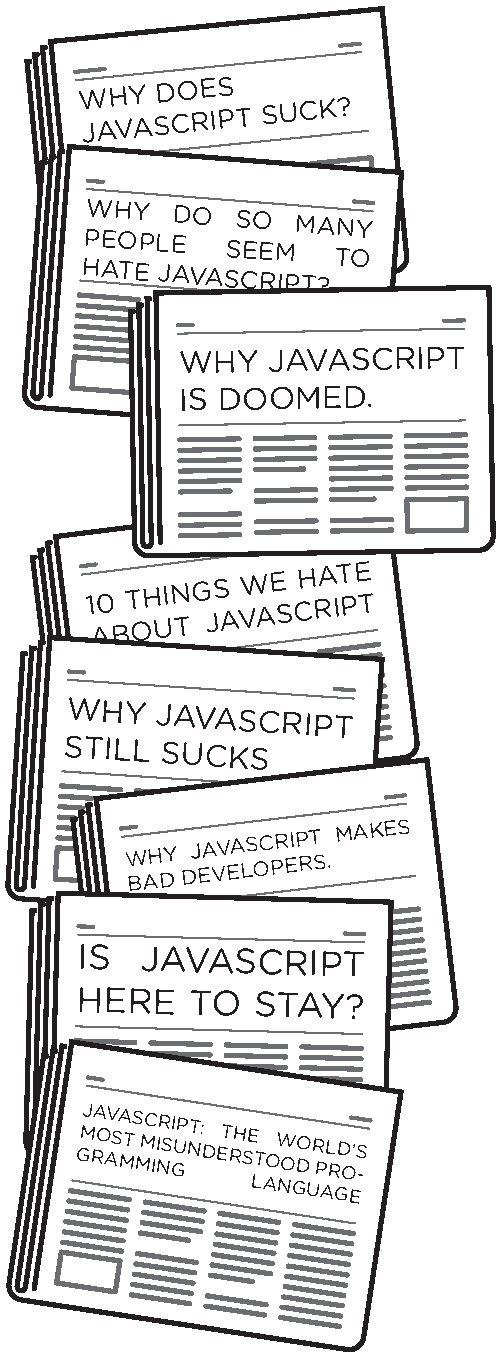
\includegraphics[width=0.3\textwidth]{../resources/javascript-hate.pdf}%
}

The web acts as a catalyst in the interaction between the community and the industry.
Because of its position in the web, Javascript is slowly becoming the main language for web development.
The next paragraph present its evolution in the industry and the community.


\subsubsection{The Ugly Duckling}

\illustration{the ugly duckling}

\cit{There are only two kinds of languages: the ones people complain about and the ones nobody uses}%
{B. Stroustrup\ftnt{http://bit.ly/stroustrup-quote}}


% Javascript was created by Brendan Eich at Netscape around May 1995, and released to the public in September.
% At the time, Java was quickly adopted as the default language for web servers development, and everybody was betting on pushing Java inside the browser as well.
% The history proved them wrong\footnote{Except for mobiles, with the success of Dalvik Android.}.

Javascript was released as a scripting engine in Netscape Navigator around September 1995 and later in its concurrent, Internet Explorer.
The differences between the two implementations forced Web pages to be designed for a specific browser.
This competition was fragmenting the Web.
To stop this fragmentation, Netscape submitted Javascript to ECMA International for standardization in November 1996.
ECMA International released  ECMAScript -- or ECMA-262 -- the first standard for Javascript in June 1997. %, to which all browsers should refer for their implementations.

The initial release of Javascript was designed by Brendan Eich within 10 days, and targeted unexperienced developers.
For these reasons, the language was considered poorly designed and unattractive by the developer community.


% {\fontfamily{phv}\fontseries{l}
% \fontsize{10pt}{10pt}\selectfont
% Why does Javascript suck?\ftnt{http://whydoesitsuck.com/why-does-javascript-suck/}
% Is Javascript here to stay?\ftnt{http://www.javaworld.com/article/2077224/learn-java/is-javascript-here-to-stay-.html}
% Why Javascript Is Doomed.\ftnt{http://simpleprogrammer.com/2013/05/06/why-javascript-is-doomed/}
% Why JavaScript Makes Bad Developers.\ftnt{https://thorprojects.com/blog/Lists/Posts/Post.aspx?ID=1646}
% JavaScript: The World's Most Misunderstood Programming Language\ftnt{http://www.crockford.com/javascript/javascript.html}
% Why Javascript Still Sucks\ftnt{http://www.boronine.com/2012/12/14/Why-JavaScript-Still-Sucks/}
% 10 things we hate about JavaScript\ftnt{http://www.infoworld.com/article/2606605/javascript/146732-10-things-we-hate-about-JavaScript.html}
% Why do so many people seem to hate Javascript?\ftnt{https://www.quora.com/Why-do-so-many-people-seem-to-hate-JavaScript}
% }

But this situation evolved drastically since.
All web browsers include a Javascript interpreter, making Javascript the most ubiquitous runtime \cite{Flanagan2006}.
This position became an incentive to make it fast (V8, ASM.js) and convenient (ES6, ES7).
Any Javascript code in the browser is open, allowing the community to pick, improve and reproduce the best techniques \ftnt{http://bit.ly/coding-horror-view-source}.
Javascript is distributed freely, with all the tools needed to reproduce and experiment on the largest communication network in history.
And since 2009, it came back on the server\footnote{True hipsters used Server-Side Javascript before it was cool. \url{http://bit.ly/mdn-server-side-javascript}} with Node.js.
This omnipresence became an advantage.
It allows to develop and maintain the whole application with the same language.
All these reasons made the popularity of the Web and Javascript.

% \paragraph{Rising of the unpopular language}

\subsubsection{The Rise of Javascript}

\cit{When JavaScript was first introduced, I dismissed it as being not worth my attention. Much later, I took another look at it and discovered that hidden in the browser was an excellent programming language.}%
{Douglas Crockford\ftnt{http://bit.ly/crockford-quote}}

Javascript was initially used for short interactions on web pages.
% The typical usage was to pre-validate forms on the client to avoid wasting bandwidth with wrongly formated requests to the server.
% This situation hugely improved since the beginning of the language.
Nowadays, there are a lot of web-based applications replacing desktop applications, like mail client, word processor, music player, graphics editor\ldots

ECMA International stimulated this progression by releasing several versions to give Javascript a more complete and solid base as a programming language.
% The third version contributed to give Javascript a more complete and solid base as a programming language.
% From this point on, the considerations for Javascript kept improving.
Moreover, % in 2005, James Jesse Garrett released \textit{Ajax: A New Approach to Web Applications} \cite{Garrett2005}.
Asynchronous Javascript And XML (Ajax) allows to dynamically reload the content inside a web page, hence improving the user experience \cite{Garrett2005}.
It allows Javascript to develop richer applications inside the browser, from user interactions to network communications.
% The first web applications to use Ajax were Gmail, and Google maps\footnote{A more in-depth analysis of the history of Ajax, given by late Aaron Swartz \url{http://www.aaronsw.com/weblog/ajaxhistory}}.
The community released some frameworks to assist the development of these larger applications.
Prototype\ftnt{http://prototypejs.org/} and DOJO\ftnt{https://dojotoolkit.org/} are early famous examples, and later jQuery\ftnt{https://jquery.com/} and underscore\ftnt{http://underscorejs.org/}.

\illustration{Javascript with superpowers}

Since 2004, the Web Hypertext Application Technology Working Group\ftnt{https://whatwg.org/} worked on the fifth version of the HTML standard.
The name is misleading, it is really about giving Javascript superpowers like geolocation, storage, audio, video, and many mores.
The simultaneous releases of HTML5, ECMAScript 5 and V8, around 2009, represent a milestone in the development of web-based applications.
% Around the same time, Google released the Javascript interpreter V8 for its browser Chrome, improving drastically the execution performance.
Javascript became the \textit{de facto} programming language to develop on this rising application platform that is the Web\ftnt{http://blog.codinghorror.com/javascript-the-lingua-franca-of-the-web/}.
The main events in the history of Javascript presented in the previous chapters are summariezed in figure \ref{fig:js-timeline}.

\begin{figure}
  \bigfig{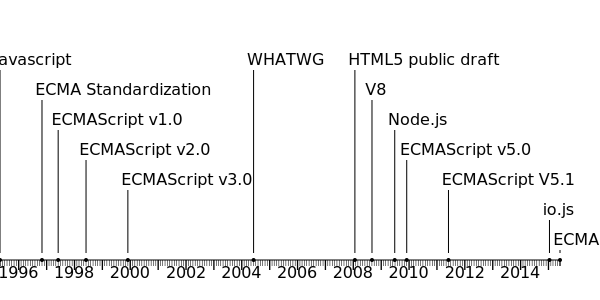
\includegraphics[width=\figurewidth]{../resources/javascript-timeline.pdf}}
  \caption{Javascript timeline}
  \label{fig:js-timeline}
\end{figure}


\separator

Javascript is now widely used on the web, in open source projects, and in the software industry.
With the increasing importance of client web applications, Javascript is assuredly one of the most important language in the times to come.
Especially that Javascript now allows to build the server side of web applications as well.
% The next paragraphs present the event-loop model used to develop Javascript web applications, both client and server-side.
The next section presents the realities and technical challenges to assure the performance of web applications against billions of users.

% \subsubsection{Event-Loop Execution Model} \label{chapter2:web-as-a-platform:javascript:event-loop}

% \nt{Reduce the event-loop explanation to the bare minimum, the definitions of callbacks and promises should be in the state of the art. It only need to present briefly how the event-loop works to understand the problem}

% Javascript is often associated with an event-based paradigm to react to concurrent user interactions.
% In 2009, Joyent released Node.js to build real-time web applications with this paradigm.
% It is a server-side implementation of Javascript based on an event-loop.
% This event-based paradigm proved to be very efficient as well for a web application to react to concurrent requests.
% This section presents the event-loop execution model, and the advantages of Javascript for this paradigm.

% The event-loop efficiency comes from non-blocking communications, asynchronous execution, and cooperative scheduling.
% It relies on a queue storing the messages received asynchronously.
% The loop executes tasks previously defined to process these messages one after the other.
% Each task can initiate new communications, leading in turn to the queuing of more messages, which trigger more tasks, and so on.
% Each task is executed atomically and exclusively, until it yields execution to continue with the next task in queue.

% \nt{TODO schema of an event-loop}

% \paragraph{Callbacks}

% In Javascript, the asynchronous communications are initiated by function calls.
% The callee immediately returns to avoid the caller to wait for the result.
% The task to process the result of the communication, and to continue the execution afterward, is a function passed as an argument to the callee.
% This function is named a callback or a continuation.
% A callback is a function passed as an argument to a callee.
% It is a continuation if the callee calls it to transfer the control back to the caller without the need for synchronization.

% In this execution model, the control flow follows the asynchronous function calls and callbacks.
% It organizes the execution of callbacks causally, one after the other, similarly to a pipeline.
% Indeed, the input stream of data flows through a sequence of callbacks until the application outputs it.
% In this model, callbacks are the atoms of the asynchronous execution flow control.
% The next paragraph presents a more elaborate form of control.

% \paragraph{Promises}

% Since the asynchronous execution flow became more complicated on larger web application, many projects proposed improved asynchronous execution controls on top of callbacks.
% The ECMAScript specification proposes Promises for such purpose.
% It arranges sequences of causally related callbacks into cleanly organized pipelines of callbacks communicating their results to the next.

% \paragraph{Closures}

% Because callbacks can be passed as an argument, they are first class citizen and imply higher-order programming. %, which is part of functional programming.
% % Javascript features higher-order functions.
% For a callback to continue the execution without needing synchronization with the caller, it needs to have access to the initial context of the caller.
% This context is linked with the function when passed to the callee.
% The association of a function and its initial context is called a closure.

% Higher-order programming is convenient for developers, as they allow great modularity in the implementation through \textit{e.g.} inversion of control.
% It is presented in further details in section \ref{chapter3:software-maintainability}.
% However, because the contexts are passed, and shared all over the implementation, this programming model needs a global memory for coordination.
% A global memory is problematic to increase the concurrency of the execution.

% This section presented Javascript as the language of the web, and its programming model.
% The next section presents the realities and technical challenges to assure the performance of web applications against billions of users.

\subsection{Highly Concurrent Web Servers} \label{chapter2:web-as-a-platform:web-servers}

% The previous section presented Javascript, the prolific language to build the Web.
% With SaaS, a web application can scale world wide with near zero latency. %, and accessing it is as simple as distributing it world wide.
% With this broad range of distribution, a new business model emerged, allowing instantaneous and free access for the user.

Since the web allows an application to scale world wide with near zero latency, the software industry needed innovative solutions to cope with large network traffic.

\illustration{busy web servers}

% \subsubsection{Scalable Concurrency}

The Internet allows communication at an unprecedented scale.
There is more than 16 billions connected devices, and it is growing fast\ftnt{http://bit.ly/cisco-connection-counter} \cite{Hilbert2011}.
A large web application like google search receives about \num{40000} requests per seconds\ftnt{http://bit.ly/google-search-statistics}.
Such a Web application needs to be highly concurrent to manage this amount of simultaneous requests.
In the 2000s, the limit to break was 10 thousands simultaneous connections with a single commodity machine\ftnt{http://bit.ly/c10k-problem}.
In the 2010s, the limit is set at 10 millions simultaneous connections\ftnt{http://bit.ly/c10m-problem}.
With the growing number of connected devices on the internet, concurrency is a very important property in the design of web applications.

\subsubsection{Event-driven Execution Model} \label{chapter2:web-as-a-platform:javascript:event-loop}

Javascript is often associated with an event-driven paradigm to react to concurrent user interactions.
% In 2009, Joyent released Node.js to build real-time web services with this paradigm.
% It is a server-side implementation of Javascript based on an event-loop.
This paradigm proved to be very efficient as well for a web application to react to concurrent requests.
In 2009, Joyent released Node.js to build real-time web applications with this paradigm.
% This section presents the event-loop execution model, and the advantages of Javascript for this paradigm.

\begin{figure}[h!]
  \textfig{
    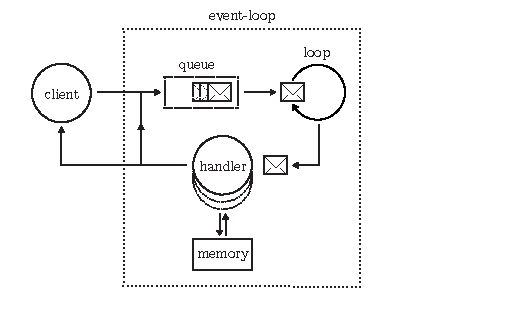
\includegraphics[width=0.7\linewidth]{../resources/event-loop.pdf}
    \caption{Event-driven execution model}
    \label{fig:event-loop}
  }
\end{figure}

The event-driven execution model is presented in figure \ref{fig:event-loop}.
At reception, each request from a client queues an event waiting to be processed.
A loop unqueues these events one at a time, and runs the appropriate handler to process them.
To process an event, a handler can query external resources, which respond asynchronously by queuing additional events.
For each query, the querying handler specifies a new handler - called continuation - to process the additional event.
Alternatively, a handler can respond directly to the client, ending this chain of asynchronous events.

% The event-loop efficiency comes from non-blocking communications, asynchronous execution, and cooperative scheduling.
% It relies on a queue storing the messages received asynchronously.
% The loop executes tasks previously defined to process these messages one after the other.
% Each task can initiate new communications, leading in turn to the queuing of more messages, which trigger more tasks, and so on.
% Each task is executed atomically and exclusively, until it yields execution to continue with the next task in queue.

This execution model allows high concurrency.
It is required to respond to a high number of users simultaneously.
Additionally, this concurrency needs to be scalable to adapt to the growth of audience. %, as explained in the next paragraph.

\paragraph{Scalability}

% because of its popularity.
% The importance of the average traffic softens the occasional spikes.
The traffic of a popular web application such as Google search remains stable, while the traffic of a less popular web application is much more uncertain.
% For example, it might become viral when it is efficiently relayed in the media.
Moreover, the load of the web application grows with its user base.
The available resources need to increase as well to meet this load.
For stable traffic, this growth is steady enough to plan the increase of resources ahead of time.
But for unstable traffic, it is erratic and challenging to meet.

An application is scalable, if it is able to spread over resources proportionally as a reaction to its load to use these resources efficiently.
It is a desirable property, as it helps to meet the growth, without spending time to manually spread the application on available resources to react to this erratic growth.
% It allows to use  provisionning of Platform as a Service (PaaS) solutions.

\paragraph{Time-slicing and Parallelism}

Concurrency is achieved differently on hardware with a single or several processing units.
On a single processing unit, the tasks are executed sequentially, interleaved in time.
While on several processing units, the tasks are executed simultaneously, in parallel.
Parallel executions uses more processing units to reduce computing time over sequential execution.

If the tasks are independent, they can be executed in parallel as well as sequentially.
This parallelism is scalable, as the independent tasks can stretch the computation on the resources so as to meet the required performance.
However, the tasks within an application need to coordinate together to modify the application state.
This coordination limits the parallelism and imposes to execute some tasks sequentially.
It limits the scalability.
The type of possible concurrency, sequential or parallel, is defined by the interdependencies between the tasks.
The pipeline execution model avoid interdependencies between the tasks to assure their parallel execution.

\subsubsection{Pipeline Execution Model}

The pipeline execution model, presented in figure \ref{fig:pipeline}, is composed of isolated stages communicating by message passing to leverage the parallelism of a multi-core hardware architectures.
It is well suited for streaming application, as the stream of data flows from stage to stage.
Each stage has an independent memory to hold its own state.
As the stages are independent, the state coordination between the stages are communicated along with the stream of data.

\begin{figure}[h!]
  \textfig{
    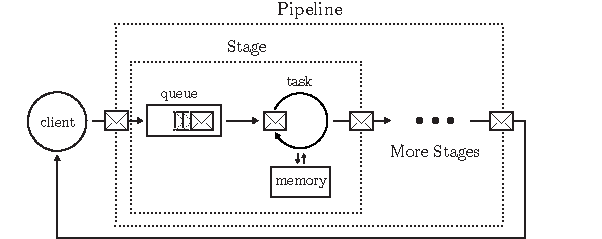
\includegraphics[width=0.8\linewidth]{../resources/pipeline.pdf}
    \caption{Pipeline execution model}
    \label{fig:pipeline}
  }
\end{figure}

The execution model of each stage is organized in a similar fashion than the event-driven execution model presented previously.
It receives and queues messages from upstream stages, processes them one after the other, and outputs the result to downstream stages.
The pipeline architecture is different as each task is executed on an isolated stage.
Whereas in the event-driven execution model, all handlers share the same queue, loop and memory store.
This difference is illustrated in figure \ref{fig:models-difference}.
The isolation of memory in the pipeline execution model impacts the productivity of its programming model.

% The previous section presented the event-loop execution model used by Javascript.
The event-driven requires a global memory to assure development productivity.
Whereas the pipeline execution model assures the isolation between the tasks to assure efficiency.
The former presents limited scalability, whereas the latter does not.
% The event-loop is constrained within time-slicing concurrency to assure this coordination.
This thesis argues that there exists an equivalence between the event-driven model and the pipeline execution model.
Before drawing this equivalence, the next section details further the incompatibility between the two programming model and the resulting economical consequences.

% \begin{figure}[h!]
%   \centering
%   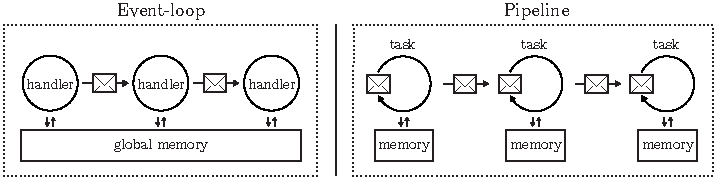
\includegraphics[width=0.8\linewidth]{../resources/models-difference.pdf}
%   \caption{Comparison of the two memory models}
%   \label{fig:models-difference}
% \end{figure}

\begin{figure}[h!]
  \centering\dualfig{
    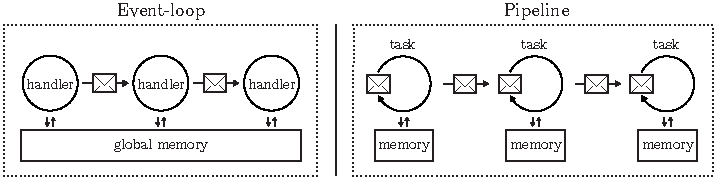
\includegraphics[page=1]{../resources/models-difference.pdf}}{
    \includegraphics[page=2]{../resources/models-difference.pdf}}{
    \caption{Comparison of the two memory models}
    \label{fig:models-difference}
  }
\end{figure}


% \begin{figure}[h!]
%   \centering
%   \begin{minipage}{0.49\textwidth}
%     \centering
%     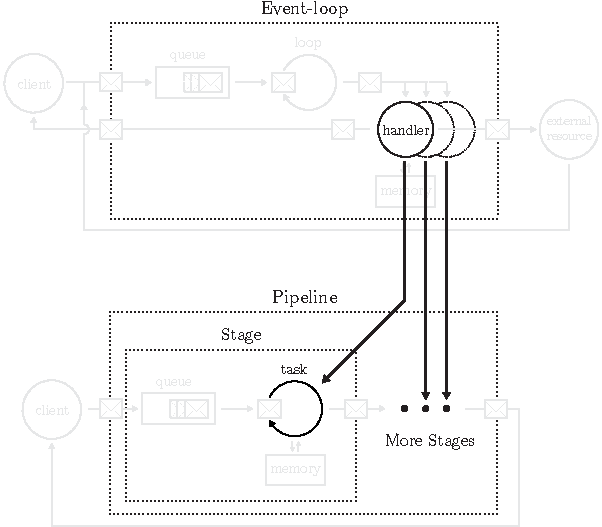
\includegraphics[width=\linewidth]{../resources/run-equivalence.pdf}
%     \label{fig:run-equivalence}
%     \caption{Execution equivalence}
%   \end{minipage}
%   \hfill
%   \begin{minipage}{0.49\textwidth}
%     \centering
%     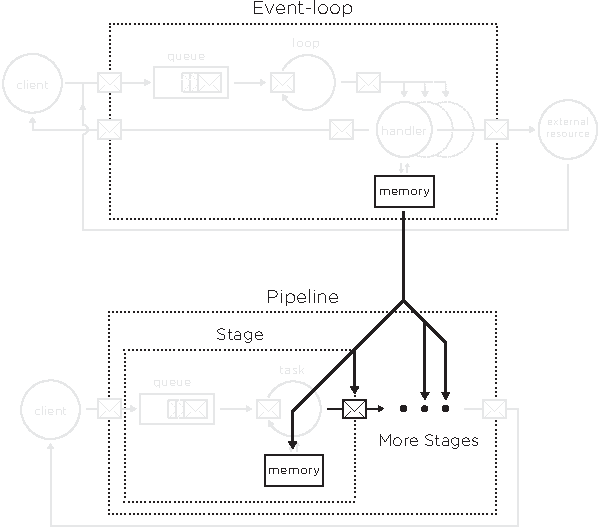
\includegraphics[width=\linewidth]{../resources/mem-equivalence.pdf}
%     \label{fig:mem-equivalence}
%     \caption{Memory Equivalence}
%   \end{minipage}
% \end{figure}

%% \separator

%This section presented two execution models to build web applications, the event-loop and the pipeline.
% It presented briefly their similitudes and differences.
